\section{Vision Transformer}\label{sec:vision-transformer}
In order to understand the paper \emph{Surgical-Dino} being examined in this report, the first thing to understand is the algorithm used as the backbone of the suggested model which are Vision Transformers (ViTs).
ViTs, as introduced by Dosovitskiy et al. in 2020~\cite{Dosovitskiy2020}, build on the work of Vaswani et al.~\cite{Vaswani2017}, adapting the transformer architecture, which until then were mostly used for natural language processing (NLP), for image classification. 
ViTs leverage the transformer's strengths in handling sequential data by splitting an image into a sequence of smaller, e.g. $16\times16$ pixel patches, and processing them through the transformer architecture just like tokens as explained below.
\begin{figure}
    \centering
    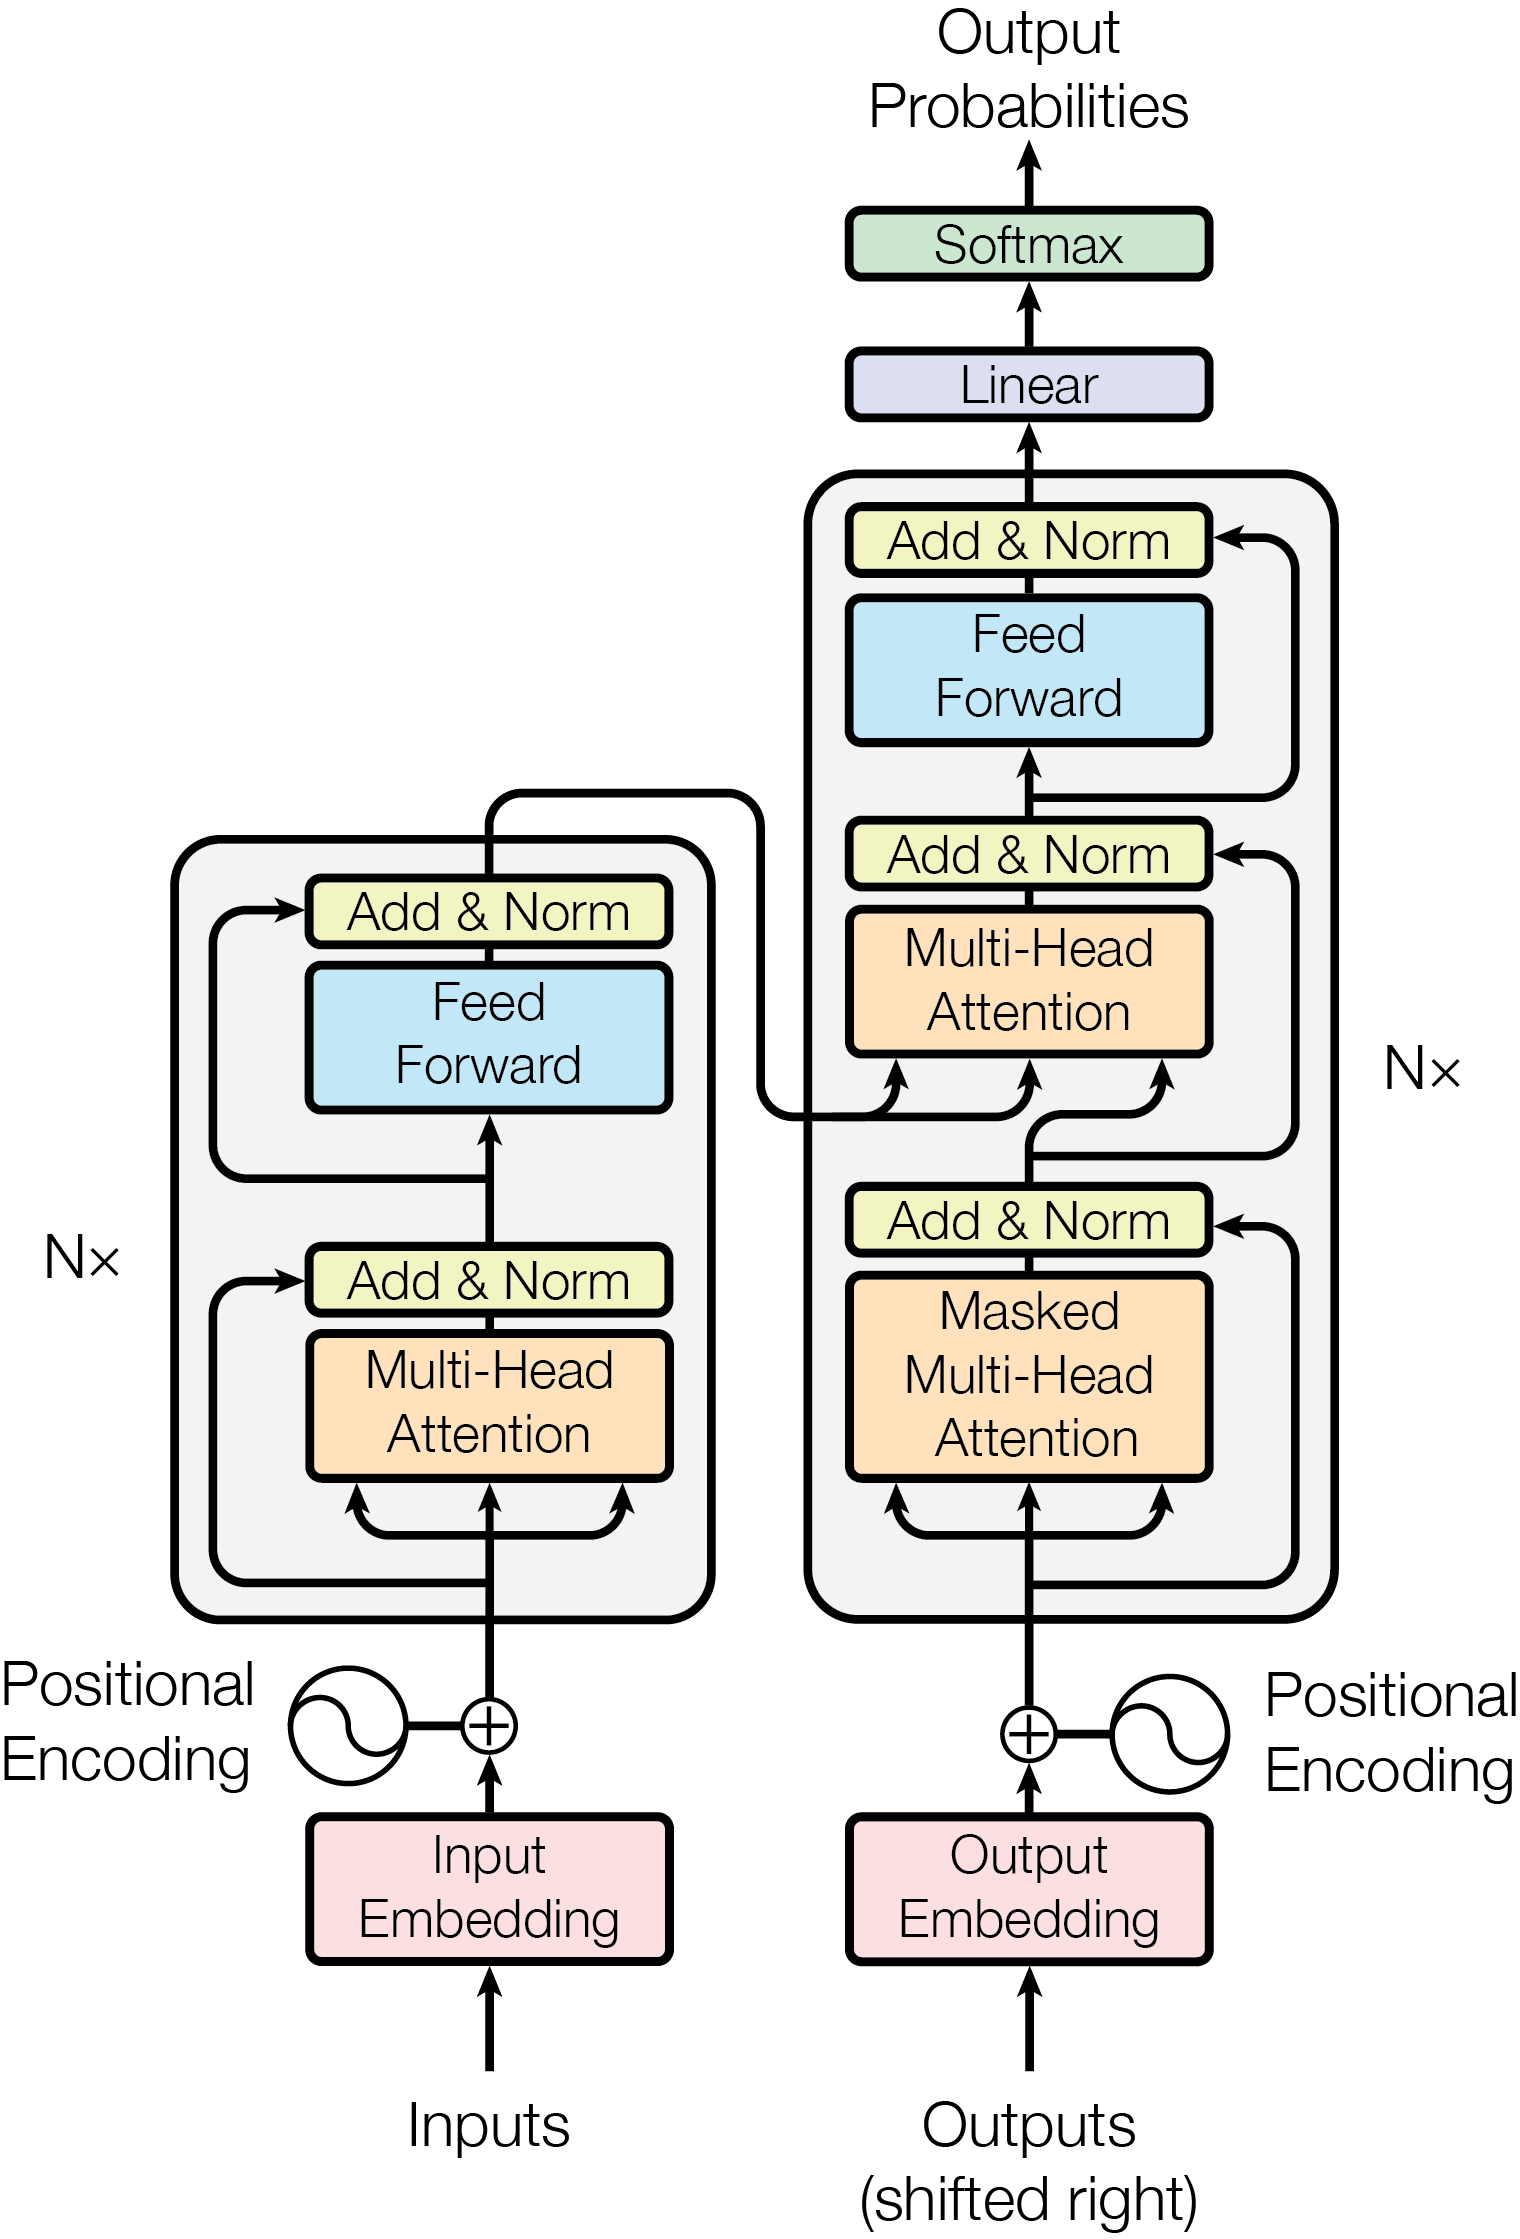
\includegraphics[width=0.3\textwidth]{images/TransformerArchitectureVaswani2017TransformerPage3.png}
    \caption[The original transformer architecture]{The transformer architecture (image from~\cite{Vaswani2017})}\label{fig:transformer}
\end{figure}

The advantage of ViTs over conventional Convolutional Neural Networks (CNNs), which most previouse state-of-the-art (SOTA) models for computer vision tasks were based on, is the ability to not only capture local features in a hirachical manner, but also to capture global context information of the image not necessarily being in the same region of the image~\cite{Khan2023}.
Additionally they seem to scale better with the amount of data and paramters compared with popular CNN architectures, but are tending to perform worse when trained on smaller datasets from scratch~\cite{Han2023}.
The original transformer architecture, designed for machine translation, consists of an encoder-decoder structure that processes input sequences through \emph{Embedding Layer}, \emph{Positional Encoding}, \emph{Encoder} containing \emph{attention mechanisms} and \emph{MLPs}, and a \emph{prediction head}. 
The following describes these components in the context of the original transformer architecture which is illustrated in Figure~\ref{fig:transformer}.

\textbf{Embedding Layer:} To ingest a sequence into a transformer, it is first split into smaller pieces called tokens, which can be words, subwords, or characters, and are then mapped into continuous vector representations called \emph{token vectors}.
The goal is to split the sequence in as few üarts as possible while staying flexible for new unseen data. 
These \emph{token vectors} form the columns of the \emph{Embedding Matrix}.

\textbf{Positional Encoding:} Following the embedding a \emph{positional encoding matrix} is added to the \emph{Embedding Matrix}, which gives the model a hint of the order of the tokens in the sequence. 
This is needed as Transformers do not have an inductive bias about token order, unlike predecessors like Recurrent Neural Networks (RNNs)~\cite{Salehinejad2018} or Long Short-Term Memory (LSTM) networks~\cite{Hochreiter1997}.

\textbf{Encoder:} Typically an \emph{Encoder} consists of multiple \emph{Transformer Blocks} out in sequentialy which are described in the following: The \emph{Embedding Matrix} with the \emph{Positional Encoding} added, is then processed by a \emph{Multi-Head Attention} consisting of $h$ \emph{Attention Heads}.
The original paper achieved good results with $h=8$.
An Attention head first runs the \emph{Embedding Matrix} through three learnable linear layers $W^Q, W^K \&\, W^V$ in parallel, producing three matrices: \emph{query matrix} $Q$, \emph{key matrix} $K$, and \emph{value matrix} $V$ each $\in \mathrm{R}^{d_{\text{model}\times d_k}}$ with $d_{\text{model}}$ being the length of a token vector (512 in the original paper) and $d_k = \frac{d_{\text{model}}}{h}$. 
These terms are analogous to database operations, where the query matrix is the search query, the key matrix is the database, and the value matrix is the data in the database. 
These terms try to convey the intuition behind the attention mechanism.
These matrices are processed by one or more \emph{Attention Heads} as shown in Equation~\ref{eq:attention} to calculate the attention score using the Scaled Dot-Product Attention method. 
First the query matrix $Q$ and the transposed key matrix $K$ is multiplied, devided by the square of the dimension of the matrices $d_k$ and then normalized using softmax to prevent exploding gradients.
This dot product is the \emph{Attention Matrix} of dimension $d_{\text{model}}\times d_{\text{model}}$ which contains the \emph{Attention Scores} which can be interpreted as probabilities of how much a certain token is correlated to another token \textbf{Explained in a good manner here~\cite{Han2023}}. 
This \emph{Attention Matrix} then multiplied with the value matrix $V$ resulting in the weighted value matrix.
Having $h$ attention heads leads to $h$ weighted value matrices which are concatenated and processed by a final linear layer $W^O \in \mathrm{R}^{hd_k \times d_{\text{model}}}$ which transformes the outputs back to the dimension of the \emph{Embedding Matrix}.
This transformed \emph{Embedding Matrix} then is added to the unmodified input of the Transformer Block, which is called the \emph{Skip Connection}.     
\begin{equation}
    \text{Attention}(Q, K, V) = \text{softmax}\left(\frac{QK^{T}}{\sqrt{d_{k}}}\right)V
    \label{eq:attention}
\end{equation}

\textbf{Decoder:} The original Transformer architecture includes an encoder-decoder structure, where the encoder processes the input sequence and the decoder generates the output sequence token by token. While both encoder and decoder consist of the same building blocks, the decoder uses a masked multi-headed attention mechanism, zeroing out the lower left triangle of the attention matrix containing the attention scores to prevent the model from attending to future tokens. 
Following that a multi-head cross attention was applied connecting the output of the encoder with the decoder.
Since then works such as the BERT framework by Devlin et al.~\cite{Devlin2018} have shown that the decoder is not inherently needed for tasks like language translation, or text generation allowing for a simplified \emph{Encoder Transformer} architecture.

\textbf{Prediction Head:}
Following the \emph{Encoder} and \emph{Decoder} blocks a usual MLP follows doing the job the network is trained to do, so either classification, such as the next token, a class the sequence is belonging to or processing the processed input sequence in any other way.
These prediciton heads often only process one or more specific tokens, either the last sequence token as in the original transformer, or a prepending class token as done in the ViT or BERT architectures.

This methodology is largely copied by the ViT architecture, though slightly adapted as shown in Table~\ref{app:CompViT}.

The ViT is first trained on a comparably large dataset with a large number of classes. 
Following this the  and then is trained for a downstream classification task on a smaller dataset with a higher resolution. 

Using this simplified Transformer architecture, as visualized in Figure~\ref{fig:vit}, ViTs have demonstrated superior performance over state-of-the-art convolutional neural networks (CNNs) in several image classification tasks~\cite{Mauricio2023}. 
Since the original ViT paper, many more use cases beyond image classification have emerged for Transformers in the computer vision field. 
For example, ViTs have been successfully applied in anomaly detection where they identify unusual patterns in manufacturing images, and in medical imaging~\cite{Ranftl2021} for monocular depth estimation in the endoscopy domain. 
These applications benefit from ViTs' ability to analyze the global context of images, demonstrating their potential in diverse and critical domains,~\cite{Jamil2023}.
Despite requiring significantly more training data than previous state-of-the-art CNN architectures, ViTs effectively leverage the transformer architecture to surpass the previous state of the art, highlighting the importance of unsupervised pre-training on large datasets and the flexibility of transformers in processing different types of data beyond natural language.
\begin{figure}
    \centering
    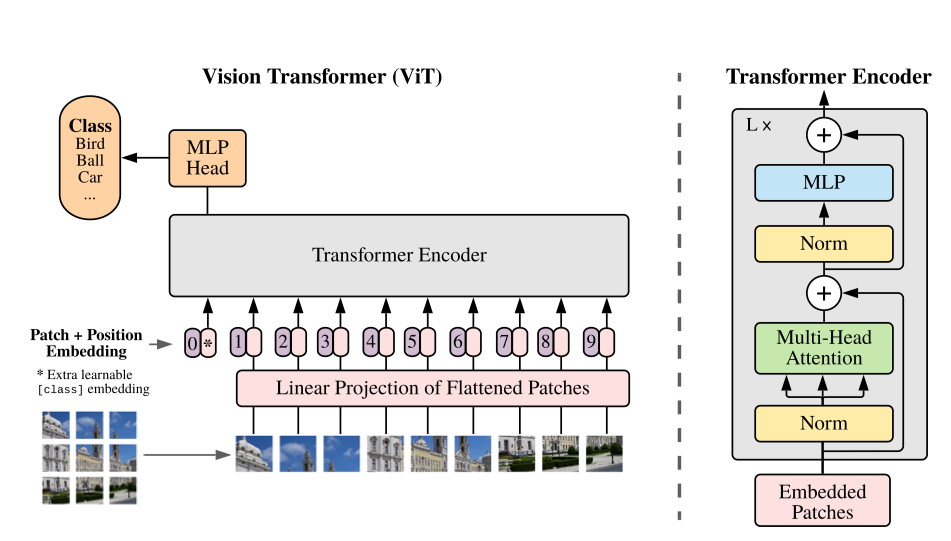
\includegraphics[width=0.8\textwidth]{images/vit_overview.png}
    \caption[The Vision Transformer architecture]{The Vision Transformer architecture (copied from~\cite{Dosovitskiy2020}).}\label{fig:vit}
\end{figure}

\section{Unsupervised Pretraining}\label{sec:unsupervised-pretraining}
Now that ViTs allow to create large scale models for computer vision tasks the need arises to train these models in an unsupervised manner in order to yield even better performance.
Unsupervised learning means the training of a network without any lables for the data, which facilitates the creation of huge datasets with millions or even billions of samples.
While these models often already are showing impressive clustering results and can be used for clustering algorithms such as K Nearest Neigbhors (KNN) or similar, usually these models are afterwards fine-tuned in a supervised manner for different downstream tasks which usually takes comparably little datasets and little computational resources to achieve state-of-the-art performance.
The overall term for these models is foundation models~\cite{Bommasani2021}.
For NLP tasks approaches such as masked language modeling, as used in BERT~\cite{Devlin2018}, or generative pretraining, as used in GPT~\cite{Radford2018}, have been successfully applied.
For Images however the methodology of predicting the next token does not make as much sense as for text, as images itself are not sequential data.

There are already several works such as ~\cite{Wei2022,Bao2021} using the same methodologie of masked input modeling as suggested for Bert~\cite{Devlin2018} which already improve the performance by several percent on the ImageNet classification dataset.
However with around $86\,\%$ accuracy there is still more room for improvement and a need to find alternative approaches.

One of these was made popular among other works by hadsell et al.~\cite{Hadsell2006} and is called contrastive learning, using siemese networks consisting of two identical networks in parallel, to learn to differentiate between similar and different images. The task to predict if the images both networks were presented with are similar, or different is called a contrastive task and is needed to prevent model collaps to a trivial solution, if the train task would be to predict the output of the other network given the same input.
This was idea was develpoed further by Chen et al.~\cite{Chen2020} in 2020 who applied contrastive learning to a ResNet50 Network.

Grill et al.~\cite{Grill2020} then introduced the Bootstrap Your Own Latent (BYOL) framework eliminating the need for negative samples to prevent model collaps by changing the way both networks udpate their weights. 
Grill et al. figured, it, to prevent model collaps, they would randomly initialize the second network, the teacher network, and freeze its weights, the student network would still while not achieving good results in down stream tasks, definitly learns meaninfull representations of the images.
To further improve this they figured that updating the teacher weights based on the moving average of the student weights would prevent the model from collapsing to a trivial solution.
This however is yet to be mathematically proven, but the authors empirically show, that the model does not collaps and intentionally made designchoices to prevent that.\textbf{dig into the reasoning they give in the paper}
The pipeline of BYOL starts with generating several augmented crops and providing each, the online and target network with a different randome augmentation of the same image.
Next both networks process their input inside a ViT Encoder, called the representation Block. 
This is followed by a few MLP for dimensionality reduction. 
The student also has another prediction MLP which introduces an asymmetry into the model, likely making the trivial solution of outputting a constant vector less likely.
Afterwards a scaled cosin similarity between the output of the online Network $q_{\theta}(z_{\theta})$ and the target network $\bar{z}'_{\xi}$ is calculated as shown in Equation~\ref{eq:byolloss}.
Afterwards the inputs of the networks are switched, so both networks get the images of the other one.
Then the cosin similarity is again calculated and the loss is calculated as the sum of both similarities and used to optimize the online networks weights.
The weights of the target netowork $\xi$ are updated as the exponential moving average of the online networks weights $\theta$ as shown in Equation~\ref{eq:byol} with $\tau$ being set to $0.99$ in the BYOL paper.
\begin{equation}
    \mathcal{L}_{\theta, \xi} \triangleq \left\| \bar{q}_{\theta}(z_{\theta}) - \bar{z}'_{\xi} \right\|_2^2 = 2 - 2 \cdot \frac{\langle q_{\theta}(z_{\theta}), z'_{\xi} \rangle}{\| q_{\theta}(z_{\theta}) \|_2 \cdot \| z'_{\xi} \|_2}\label{eq:byolloss}
\end{equation}
\begin{equation}
    \xi \leftarrow \tau \xi + (1-\tau) \theta
    \label{eq:byol}
\end{equation}

\section{DINO: Unsupervised Learning with Vision Transformers}\label{sec:dino}
\begin{figure}
    \centering
    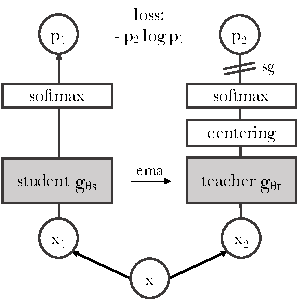
\includegraphics[width=0.5\textwidth]{dino_arch.pdf}
    \caption[The DINOv1 Architecture]{The DINOv1 Architecture showing the Student Teacher Setup. \emph{sg} stands for stop Gradient (image from~\cite{Caron2021})}\label{fig:dinov1}
\end{figure}
The \textbf{DI}sitllation with \textbf{NO} labels (DINO) framework, introduced by Caron et al. in 2021~\cite{Caron2021}, is another approach of implementing self-distillation for ViTs inspired by the findings of the BYOL paper as introduced in Section~\ref{sec:unsupervised-pretraining} and being build on by the \emph{Surgical-Dino} paper being examined in this paper.
The goal of DINO is the same as for BYOL, to train a ViT Encoder for image representation learning from scratch in an unsupervised manner for later use in downstream tasks.
The key differences from DINO to BYOL are the training task, the image augmentation, and the architecture of the student network $s$ and the teacher network $t$ which can be seen in Figure~\ref{fig:dinov1}:
\begin{itemize}
    \item \textbf{Training Task:} DINO tries to minimize the mean of the cross-entropy (Equation~\ref{eq:dino_loss}) between the student and teacher network's outputs of two different crops each.
    \item \textbf{Image Augmentation:} DINO augments the images only by cropping. DINO differentiates between two different kind of crops: Global crops contain more then $50\,\%$ of the image and local crops containing less then $50\,\%$ of the image. The teacher only gets the global crops while the student sees all the crops. This way the student has to learn the transfer from local to global.
    \item \textbf{Architecture:} The DINO framework uses a student teacher network where both the student and the teacher have the same architecture instead of having an asymetric architecture with another projection head added to the student.
\end{itemize}

\begin{equation}
    \mathcal{L} = -\sum_{x} P_{t}(x) \log P_{s}(x)
    \label{eq:dino_loss}
\end{equation}
\begin{equation}
    P_{t}(x) = \text{softmax}\left(\frac{g_{\theta_t}(x)}{\tau}\right)
    \label{eq:softmax}
\end{equation}

\TS{Information about how DinoV2 Changes}

\section{Monocular Depth Estimation}\label{sec:depth-estimation}

Monocular Depth Estimation (MDE), also known as Monocular Dense Estimation, is a discipline where, given a single image, the model learns to predict the depth of every pixel.
This task often scales depth values from 0 to 255. 
Monocular depth estimation holds significant potential in fields such as robotics, autonomous driving, and medicine and also gets more and more important for generative image and video creation. 
These areas require precise 3D representations of the environment, but sensors capable of capturing depth information can be too expensive or impractical due to space constraints or limited availability in general.

In generall there are two main approaches to monocular depth estimation: generative models e.g. based on diffusion networks and discriminative models e.g. based on CNNs or more recently hybrid models combining CNNs with Vision Transformers (ViTs) as demonstrated by works such as~\cite{Ranftl2021,Yang2024,Oquab2023}.

Recently, there has been a shift towards using hybrid models that combine CNNs with Vision Transformers (ViTs), as demonstrated by works like Ranftl et al.~\cite{Ranftl2021}. 
In these hybrid models, the ViT typically encodes the image, transforming it into feature tokens enriching them with additional information. 
These tokens are then usually processed by a CNN-based prediction head to generate a depth map.


%See DinoV2 Section 7.4 \cite{Oquab2023}
% Monocular depth estimation, also known as monocular dense estimation, is a diciplin, where, given one image, the model learns to predict the depth of every pixel, often on a scale of 0 to 255. 
% This has much potential for tasks in the field of robotic, autonomouse driving and medicin, where 3D-representation the sourounding is very important for the task at hand, but either sensors capable of capturing depth information are too expansive or it is not possible to use them due to space constraints or availability.
% To do this a lot of supervised architectures were build making especially use of CNNs and recently have bin used in hybrid with Vision Transformers in works such as from Ranftl et al.~\cite{Ranftl2021}.
% In these works usually the ViT is encoding the image and the prediction head is a CNN network processing the tokens into a depth map
% Quickly after the publication of ViT which were trained using supervised classification frameworks, methodologies emerged for unsupervised pre-training of ViTs for images.
% Pre-training in this case means, that a model is trained on a usually larger and more diverse dataset and afterwards can be finetuned for different downstream tasks.
% The inital pre training is, compared to the fine tuning, way more computationally expansive which is the why much efforts are being made to train few very big models, so called foundation models, and to derive many smaller models from them using methods such as few shot learning~\cite{Bommasani2021}.
% As these foundation models need a lot of data it is desired to train the model unsupervised, as labeled data is expensive and often not available in the quantities needed to train a model.
% This is where Dino comes into play, as it is a framework for unsupervised pretraining Vision Transformers on large datasets~\cite{Caron2021}.
% The goals by Caron et al. were to make a model learn image representations in a meaningful way, without needing any lables for the images.

% Essentially all ML algorithms are converting their input into a usually smaller representation along the line. 
% For supervised learning however, we train the model explicitly to learn a representation that e.g. is usefull for classification, so the model only learns representations for data it was trained on.
% For unsupervised learning we do not have any lables to guide the model via the loss function, so the model has to learn to encode the data in a meaningful way by itself.
% One common approach to solve this issue is to train two models in parallel where the two models learn to predict each others output given two different augmented versions of the same source image, which is known as self-distillation.
% These frameworks are often called student-teacher networks or online-target networks~\cite{Zhang2021}.
% This, however, can lead to a model collaps leading to a trivial solution where the model learns to output a constant vector all the time.
% To tackle this problem there are several methodologies, such as contrastive learning~\cite{Chen2020} or Bootstrap Your Own Latent (BYOL)~\cite{Grill2020}.

% \emph{Contrastive Learning} tackles the problem of model collaps by occasionally giving the student and teacher inputs from different source images, a so called negative pair.
% Given the two outputs of the two networks a MLP classifier predicts if the two networks were presented with images from the same source, or not. 
% This way a collaps is mitigated, as for negative pairs the outputs shoud a much higher difference, e.g. euclidian distance,  then the positive pairs, which should be closer together~\cite{Chen2020}.

% \emph{Bootstrap Your Own Latent (BYOL)}, proposed by Grill et al.~\cite{Grill2020}, does not need negtative samples to prevent the collaps, but is using loss using a momentum encoder to update the teacher networks weights $\zeta$ based on the exponential moving average of the student network's weights $theta$ as shown below.
% \begin{equation}
%     \zeta \leftarrow \tau \zeta + (1-\tau) \theta
%     \label{eq:byol}
% \end{equation}
% $\tau$ in the BYOL paper is set to $0.99$.
% Interestingly, so far it is not mathematically proven that model collapse can't happen with this approach, but empirically it did not happen for the authors of the BYOL paper~\cite{Grill2020}.

% The original Transformer architecture first was build to be trained in a supervised manner, but quickly Frameworks such as BERT~\cite{Devlin2018} introduced ways to train transformer unsupervised on large quantities of data to yield so called foundation models~\cite{Bommasani2021} which are the basis of of many more fine-tuned models for specific tasks.
% The advantage of these foundation models is, that the models can learn concepts and patterns from a much more diverse set of data and then can be fine-tuned for domains where there is either a lack of large enough datasets for machine learning, or where computational ressources are limited.
% Quickly after the publication of ViT, which was trained supervised for classification, frameworks emerged to unsupervised train ViTs for image representation learning. 
% With image representation learning it is usually meant, that a network learns to encode images in a smaller feature vector space in a meaningfull way, where similar images would have vectors very similar to each other and different images would have very different vectors.
% To solve this task unsupervised usually a student teacher network is used where the both the student and the teacher have the same architecture and the student tries to predict the output of the teacher given a similar input. 
% The Input is derived from the training image which is the rendomly augmented twice, once for the student and once for the teacher.
% This way the idea is, that the networks can actually learn to encode the image semantically and not just memorize the output for a specific input.
% The trivial solution for the network would be to output the same output for every input.
% To prevent this there are manly two approaches:
% \emph{Contrastive Learning} occasionally provides the teacher and student with different images where the goal is to maximise the distance of their representation vector~\cite{Chen2020}.
% \emph{BYOL} by Grill et al.~\cite{Grill2020} does not use a contrastive loss but instead uses a momentum encoder to update the teacher network according to the change of the student weights. 
% This helps to prevent the parameter collapse and the networks can focus on learning the semantic meaning of the images.

% While the ViT architecture was originally developed for supervised learning, its potential in unsupervised settings emerged shortly after e.g. in form of Bootstrap your own Latent (BYOL) by Grill et al.~\cite{Grill2020}.
% Pioneering works like BERT have shown how Transformers can be adapted to leverage unsupervised learning on vast datasets, creating versatile foundation models that serve as pre-trained starting points for more specialized tasks~\cite{Devlin2018, Bommasani2021}. 
% The advantage of these models lies in their ability to discern complex patterns and concepts from diverse data sources even without lables, making them ideal for as a starting point for fine-tuning the model to task specific domains with limited data or computational resources. 
% Inspired by these developments, the DINO framework applies a similar philosophy to ViTs, using self-supervised learning to distill knowledge from unlabeled image data, thus facilitating significant advancements in model performance and efficiency.

% Right out of the box the resulting ViT is already good at segmentation tasks and knn classification tasks, as the model has learned to place similar images close to each other in the latent space, similar to how similar words are placed close to each other in an embedding space when training a word embedding~\cite{Caron2021}.

% The same methodologies as used for BERT could not be applied to the ViT's due to the different structure of images and text, and how we interact with them.
% The Dino Framework by Caron et al.~\cite{Caron2021} however changed that, by introducing a untypical student teacher network.
% Usually the goal for a stundent teacher network is to use a larger already trained teacher model which is used to train a normally smaller, or at least different network to copy its outputs given the same input. 
% This is called \textbf{knowledge destillation (CHECK IF TRUE)}
% The DINO framework however is using an untrained teacher network having the same architecture as the student with the only difference in how their weights get updated, \textbf{more on this later}.

% \textbf{Student Teacher Network:} The DINO is, as already mentioned, a framework for unsupervised pretraining Vision Transformers on large datasets. 
% This is archived by using a student teacher network each having the same ViT model architectur.

% The DINO (DIstillation with NO labels) framework, proposed by Caron et al. in 2021~\cite{Caron2021}, represents a significant advancement in self-supervised learning for ViTs, as introduced in~\ref{sec:vision-transformer}, by adapting the principles of knowledge distillation in an unsupervised context for ViTs. 
% DINO facilitates the training of Vision Transformers without the need for labeled data, leveraging the concept of a teacher-student architecture where, though, instead of using a pretrained teacher to guide the student, both the teacher and student networks are trained simultaneously on the same data~\cite{Caron2021}.

% \subsection{Architectural Overview}
% DINO employs two networks: a student network and a teacher network, which share the same architecture but have different parameters. 
% The student learns to predict the softened outputs of the teacher network, effectively allowing the student to learn robust representations from the data without explicit labels. 
% The key components of the DINO architecture are detailed below:

% \textbf{Teacher Network:} The teacher's parameters are updated using an exponential moving average (EMA) of the student's parameters, ensuring stability and gradual improvement of the learned features over time. 
% The teacher network operates on multiple augmented views of the same input, promoting consistency and robustness in feature representation.

% \textbf{Student Network:} The student network learns by trying to predict the teacher's outputs. 
% This prediction is not a direct match; instead, the outputs are softened using a temperature-scaled softmax function, which helps in learning finer distinctions between the input features.

% \begin{equation}
%     P_{t}(x) = \text{softmax}\left(\frac{g_{\theta_t}(x)}{\tau}\right)
%     \label{eq:teacher_softmax}
% \end{equation}

% \begin{equation}
%     P_{s}(x) = \text{softmax}\left(\frac{g_{\theta_s}(x)}{\tau}\right)
%     \label{eq:student_softmax}
% \end{equation}

% Here, $g_{\theta_t}(x)$ and $g_{\theta_s}(x)$ are the outputs from the teacher and student networks for input $x$, respectively, and $\tau$ is the temperature parameter that controls the sharpness of the softmax distribution.

% \subsection{Loss Function}
% The objective of the student network is to minimize the cross-entropy loss between its predictions and the softened labels provided by the teacher network. This loss function encourages the student to produce similar predictions to those of the teacher, promoting consistency across different transformations of the same input.

% \begin{equation}
%     \mathcal{L} = -\sum_{x} P_{t}(x) \log P_{s}(x)
%     \label{eq:dino_loss}
% \end{equation}

% \subsection{Preventing Collapse}
% A common challenge in unsupervised learning is the issue of collapse, where the model outputs become invariant to the input data. DINO addresses this by employing centering and sharpening techniques on the teacher's outputs, which balance the model's tendency towards uniformity or dominance by a single dimension.

% \textbf{Centering:} Adjusts the teacher's outputs by subtracting the batch mean, preventing any single feature dimension from dominating.

% \textbf{Sharpening:} Adjusts the temperature of the softmax function, encouraging the model to make more confident predictions, thus maintaining diversity in the output space.

% These mechanisms ensure that DINO learns meaningful and diverse representations without collapsing to trivial solutions.

% \subsection{Implementation and Applications}
% DINO has been effectively implemented on top of existing Vision Transformer architectures and has demonstrated superior performance in several computer vision tasks, such as image classification and feature representation, without relying on labeled data. This makes DINO a powerful tool for leveraging the capabilities of Vision Transformers in an unsupervised manner.

% The successful deployment of DINO underscores the potential of self-supervised learning paradigms in reducing the dependency on labeled datasets, opening up possibilities for more data-efficient learning methods in the field of computer vision.

% \section{DINOv2: Enhancements and Innovations}



% DINOv2, introduced by Oquab et al. in 2024~\cite{Oquab2023}, builds upon the foundational concepts of DINO by implementing several significant improvements aimed at increasing robustness and efficiency in training Vision Transformers without supervision. 
% DINOv2 introduces a series of enhancements that optimize the learning process and extend the utility of the learned representations.

% \textbf{Expanded Data Utilization:} Unlike DINO, which primarily used curated datasets, DINOv2 includes an automatic pipeline for assembling a large-scale, diverse dataset from a mix of curated and uncurated sources. This approach allows for more robust feature learning that is less prone to overfitting on narrow data distributions.

% \textbf{Advanced Model Architecture:} DINOv2 employs a larger Vision Transformer model with up to 1 billion parameters, distilled into smaller models. This scale-up is facilitated by technical innovations that accelerate training and reduce memory requirements, making it feasible to train on larger datasets with extensive model parameters.

% \textbf{Loss Function Modifications:} DINOv2 modifies the loss functions used in DINO, integrating a discriminative self-supervised approach that combines the benefits of multiple pretext tasks. This integration enhances the discriminative power of the learned features across a broader range of visual domains.

% \begin{equation}
%     \mathcal{L}_{\text{DINOv2}} = \alpha \mathcal{L}_{\text{DINO}} + \beta \mathcal{L}_{\text{iBOT}} + \gamma \mathcal{L}_{\text{SwAV}}
%     \label{eq:dinov2_loss}
% \end{equation}

% Here, $\alpha$, $\beta$, and $\gamma$ are coefficients that balance the contribution of each loss component, optimizing the overall learning trajectory.

% \textbf{Training Efficiency Improvements:} Technical contributions in DINOv2 focus on reducing the computational demand. These include optimizations like faster attention mechanisms and memory-efficient training strategies that enable longer training durations and larger batch sizes without increased resource consumption.

% \textbf{Improved Robustness and Generalization:} DINOv2's training methodology significantly improves the robustness and generalization of the features it learns. This is evidenced by superior performance on a variety of computer vision tasks compared to DINO and other state-of-the-art self-supervised learning methods.

% These enhancements make DINOv2 a more powerful and versatile framework for training Vision Transformers, capable of achieving superior performance on a range of visual recognition tasks without the need for labeled data. The ability of DINOv2 to train on larger, more diverse datasets with a scalable architecture addresses some of the primary limitations of the original DINO, paving the way for broader applications in unsupervised visual feature learning.

% % \section{Dino and DinoV2}
% % As mentioned in the privious Section~\ref{sec:vision-transformer}, ViTs are work very well for tasks like image classification and have shown superior performance over state-of-the-art convolutional neural networks (CNNs) in several image classification tasks.
% % So far ViTs were mostly trained in a supervised manner and needed a lot of labeled data to achieve state-of-the-art performance.
% % As labeled training data is expensive and time consuming to generate, it is very desirable to train models in an unsupervised manner.
% % Just a year after the introduction of the Vision Transformer, Caron et al.~\cite{Caron2021} introduced an approach to achieve exactly this called DINO (DIstilled NOt labeled), which is a framework for training in theory any network capable of ingesting image data using self-distillation without labels.
% % However the paper in particular emphasizes the synergy of Dino with Vision Transformers as a good compromise between performance and computational cost.
% % Dino is a usefull framework for tasks such as segmentation, depth estimation, and object detection, as it provides a good initialization for supervised fine-tuning.


% % As explained in~\cite{Phuong2019} destillation in machine learning is a method facilitating the transfer of knowledge from one model to another using a teacher-student model approach.
% % Often the teacher is a larger complex pretrained model which is used to train a much smaller stundent model. 
% % However, in the case of Dino the teacher is a non-pretrained model being trained in parallel with the student model. 
% % This process is called self-distillation, as no pretrained model is used to inject prexisting knowledge into the student model.

% % In a teacher stundent architecture the student tries to predict the output of the teacher model.
% % In Dino the students weights get updated using the classical gradient decend approach, while the teacher model is updated using a exponential moving average of the student model weights.
% % Caron et al. figured that in order to prevent a trivial solution where both teacher and student would start outputing the same output no regard to the input, it is enough to center the output of the teacher model to a mean of 0 and to apply a sharpened softmax function to the output by applying a temperatur parameter $\tau$ called temperatur to the softmax function as shown in equation~\ref{eq:sharp_softmax}. It makes very large values even larger and very small values even smaller.

% % \textbf{Architecture}

% % Dino is trained using a classical student teacher network approach, though the teacher is not a pretrained model but a model trained in parallel to the student model.
% % The Tracher model is largely the same as the student model, but the outputs follow a normalisation applying centering subtracting the mean and running the resulting outputs thorugh a shapened softmax function as shown in equation~\ref{eq:sharp_softmax}.

% % \begin{equation}
% % q_{i} = \frac{f_{i}}{|f_{i}|_{2}} \cdot \tau
% % \label{eq:sharp_softmax}
% % \end{equation}



% % - Attention Map right after training puts much attention on the main object of the image and less on the background. This already is a good start for segmentation
% % - Dino is trained unsupervised and places, when trained, images in to a latent vector, where similar images are close to each other, similar to how similar words are embedded close to each other when training a embedding on them. This could already be used for a k-nearest neighbor approach to classify images.
% % \subsection{Depth Estimation}
% % \subsection{Segmentation}


\section{Model Fine-Tuning}\label{sec:model-fine-tuning}
Foundation Models (FMs), as defined in~\cite{Bommasani2021}, are models trained on a large variety of data using self-supervised learning sometimes even for weeks on hunderds of graphic processing units (GPUs) as e.g. the GPT3 model~\cite{Yuan2022} or the Florence CV Foundation Model by Yuan et al.~\cite{Yuan2021}.
These FMs can then fine-tuned doing few shot training, to tailor the FM to a specific task using several magnitutes less data as would be needed for training a model from scratch.
This saves a lot of computational cost and time as it often is enough to retrain only small parts of the FM, and most of the parameters/weights get frozen as well as that cost can be saved dataset which can be relativley small.
Mathematically, the straight forward way of fine-tuning a model is by retraining all parameters, which can be written as in Equation~\ref{eq:finetuning} with $W_0$ being the pretrained weights and $\Delta W$ the change in weights during fine-tuning.
This However still is relativley computationally intesive as the backpropagation has to be done for all parameters.

\begin{equation}
    W' = W_0 + \Delta W
    \label{eq:finetuning}
\end{equation}
% \textbf{DISCUSS IN GENERALL HOW PRETRAINING WORKS???}

A more efficient way of fine-tuning weight matrices is Low Rank Adaption (LoRA) as suggested by Hu et al.~\cite{Hu2021} in the context of transformer fine-tuning.
Hut et al. assume based on the the work of Aghajanyan et al.~\cite{Aghajanyan2020}, that the updated weight matrices $\delta W_n$ inside the attention heads of the transformer have a rank much lower then their dimensionality.
In order to utilize this assumption to more efficiently fine-tune a transformer the updated weight matrices $\delta W_n$ are decomposed into two matrices $A \in \mathbb{R}^{d \times r}$ and $B \in \mathbb{R}^{r \times k}$ with $r \ll d$ and $r \ll k$ as shown in equation~\ref{eq:lora}.
Hu et al. set the goal to use a maximum of 18M parameters for fine tuning the 173B parameter GPT3 model and created a grid search for optimizing the rank $r$ and which weight matrices to update.
Eventually they figured for their usecase a rank $r = 4$ and only applying updates to all key matrices $K$ and value matrices $V$ in the attention heads of the transformer performed the best.
Besides the advantage of significantly lowering the computational cost of only optimizing the $A$ and $B$ matrices, fine-tuning using LoRa does not increase inference times as the decomposed matrices are recomposed and added onto the original weight matrices $W_0$ after the fine tuning and therefor do not add any additional computation to the forward pass of the model.
\begin{equation}
    W = W_0 + BA
    \label{eq:lora}
\end{equation}

\begin{figure}
    \centering
    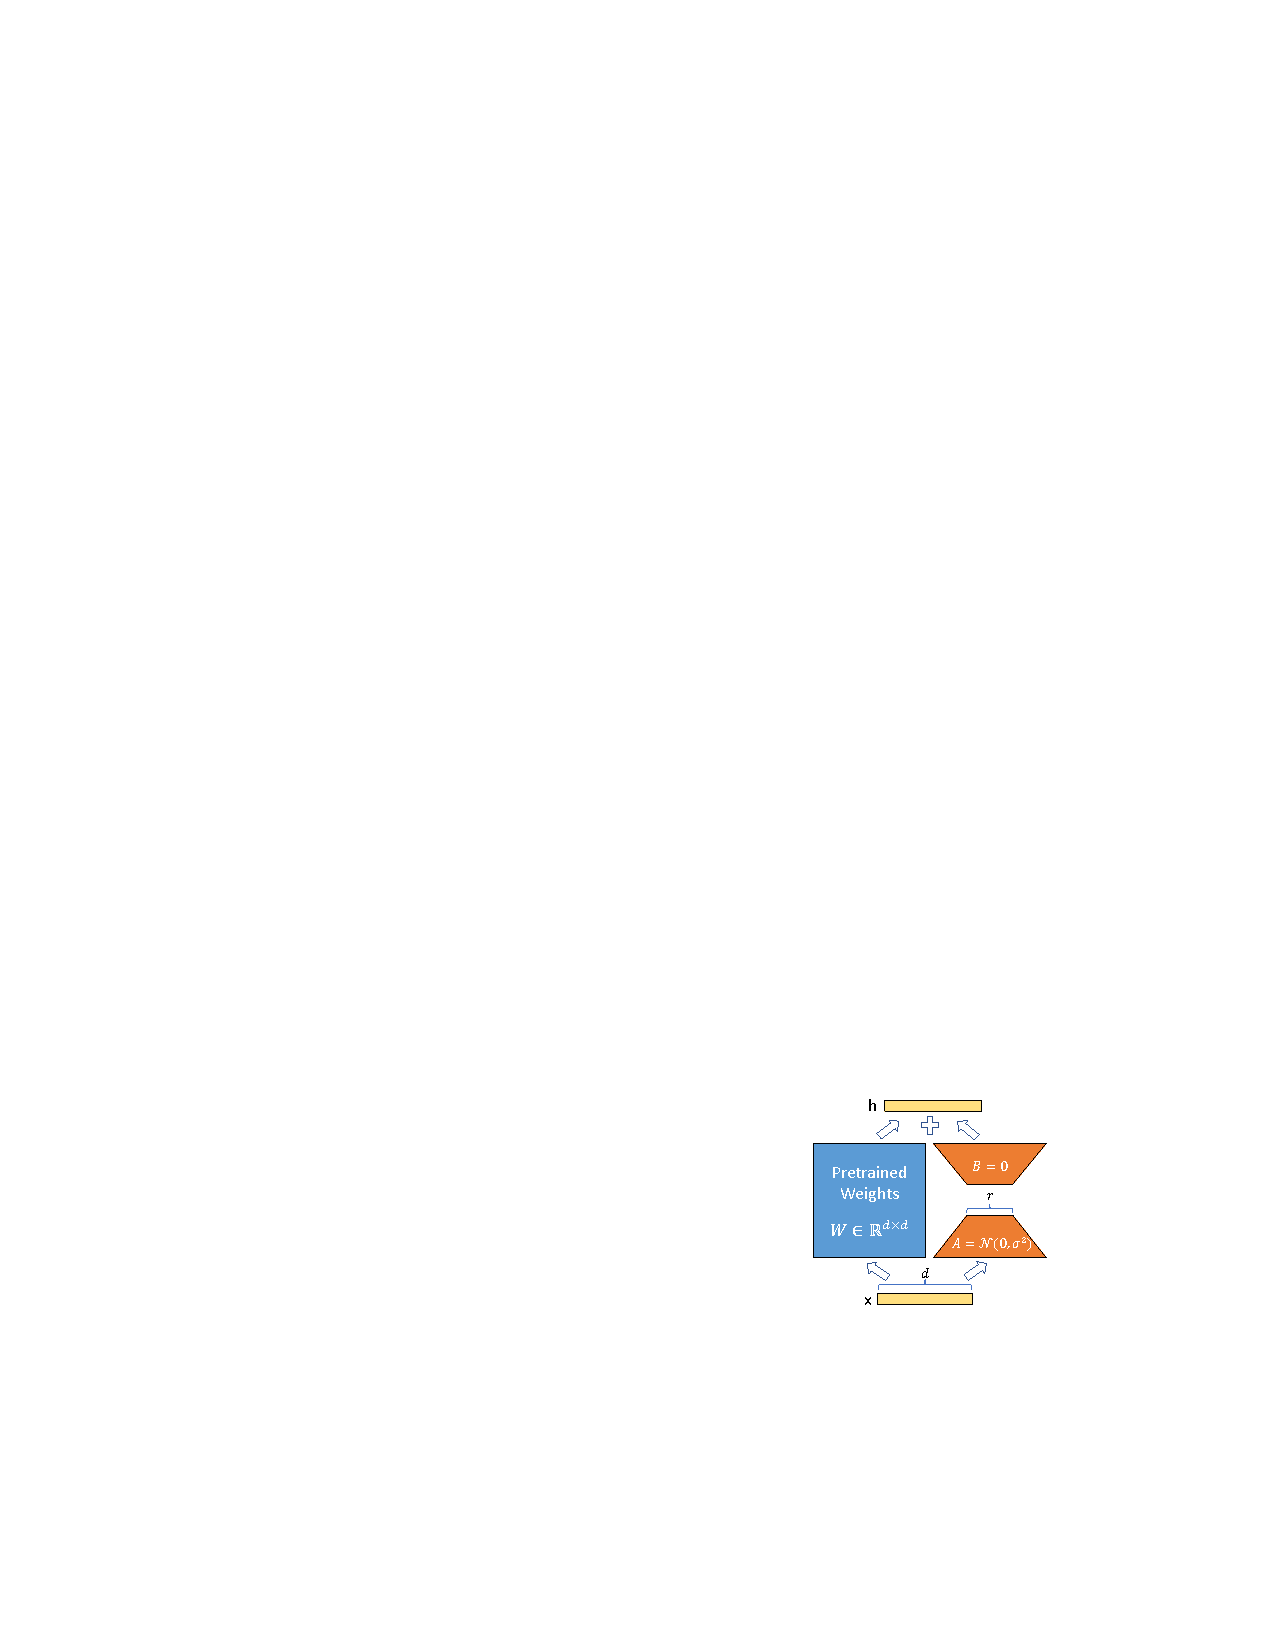
\includegraphics[width=0.5\textwidth]{images/Hu2021_LoraArch.pdf}
    \caption[LoRa Architecture]{LoRa architecture with the docomposed $\Delta W_n = AB$ and their initialization  method (graphic lifted from~\cite{Hu2021})}\label{fig:loraarch}
\end{figure}

There are more approaches for fine tuning Transformer which can be read more about here~\cite{Xin2024}.